\section{Workshop}
\subsection{Project Creation}
In order to start designing a PCB in KiCad you will first need a project! To create a project click \textbf{File, New Project, New Project} and choose a name for the project.
\\*\\*
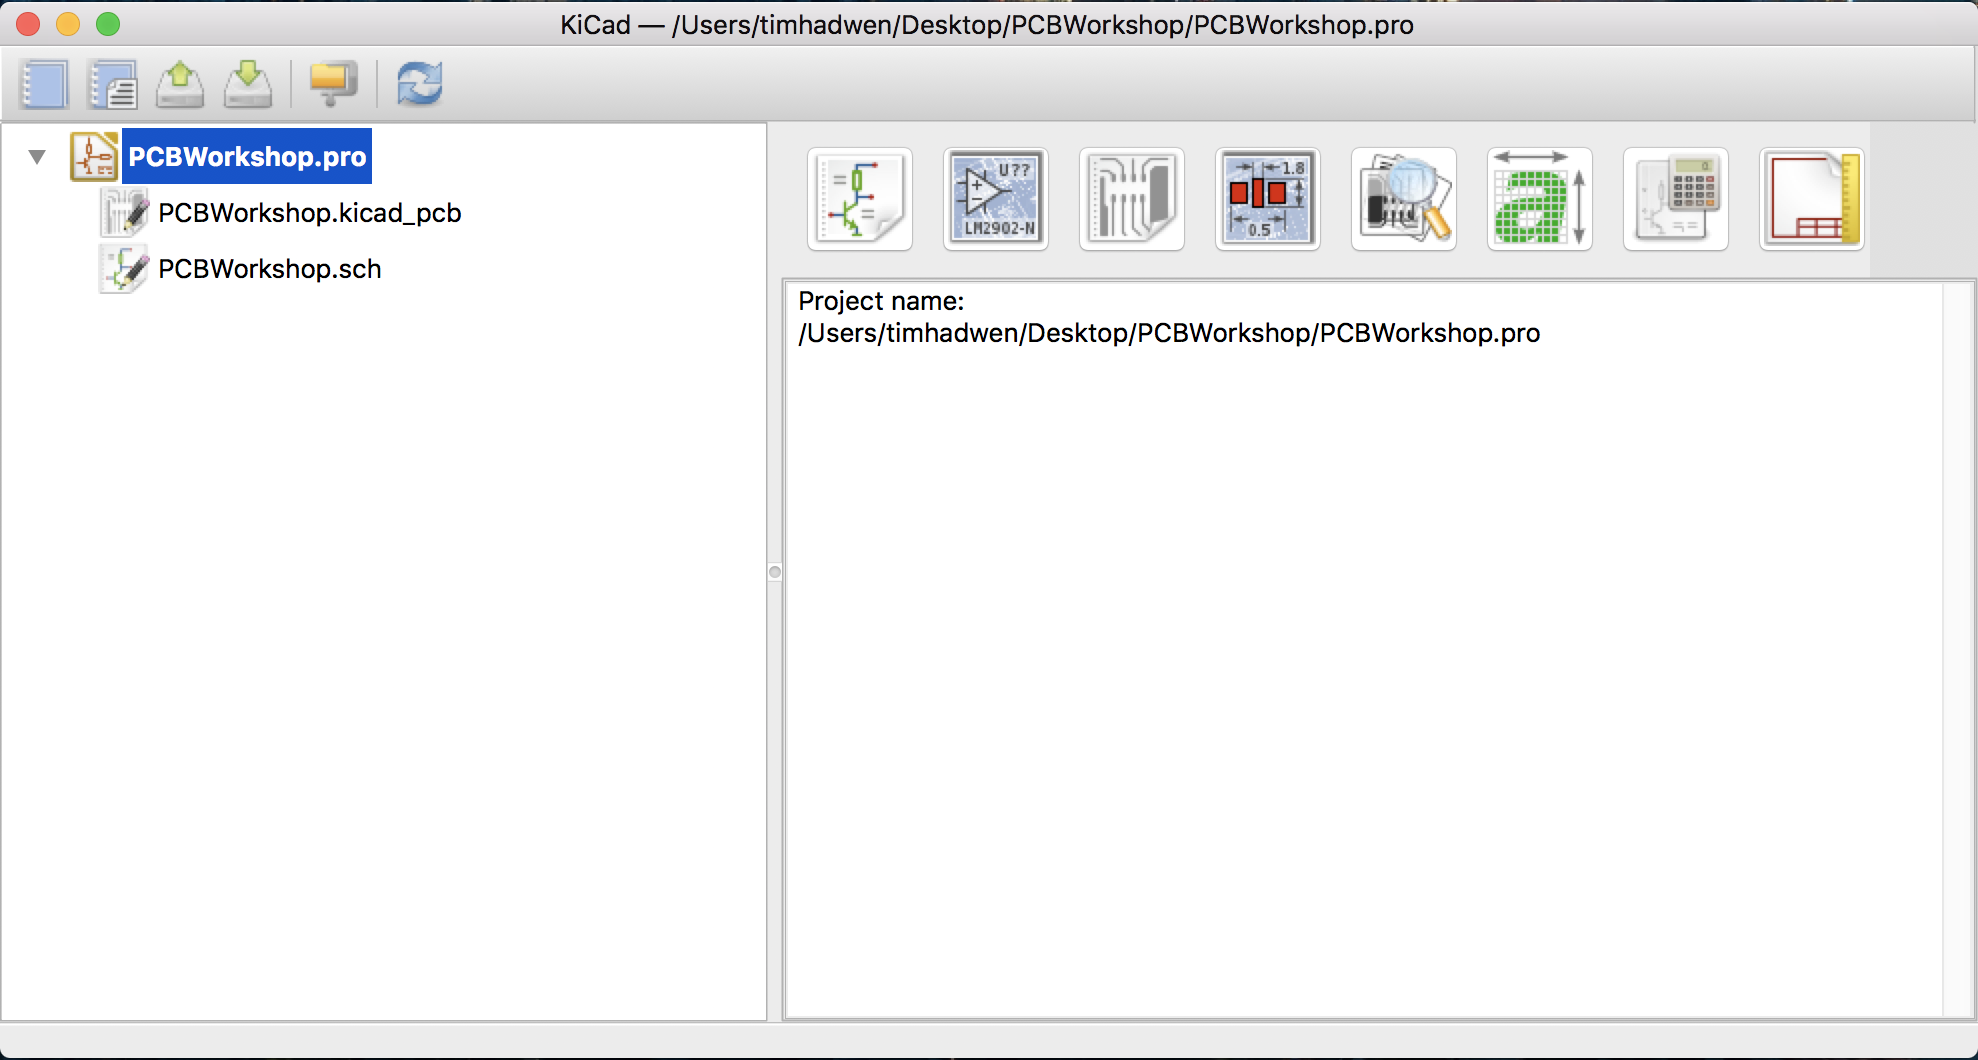
\includegraphics[width=\textwidth]{newproject}

Once the project is created we can see the project with both \textbf{kicad\_pcb} and \textbf{sch} files, these are the \textbf{Circuit Board} and \textbf{Schematic} respectively. These are all the files we need to create a PCB.\\

On this window we can also see a series of buttons on the right. These open up the programs associated with PCB Creation. The important ones (the first 4, used in this workshop) are listed below.

\begin{itemize}
	\item EESchema - Schematic Creation
	\item Schematic Library Creator - Creates schematic symbols for use in EESchema
	\item PCBNew - Layout and routing of the Circuit Board once schematic is completed
	\item PCB footprint editor - Creates the footprints for placement on the PCB
\end{itemize}

\subsection{Schematic Library Creation}
In this workshop we will only be using already existing schematic parts and therefore this section will be left out of the actual workshop and is placed here for your reading later. In most cases you will be able to find the parts you need however in the off case that you can't this is the tool for you.

\subsection{Schematic Creation}
In order to create a KiCad Schematic we must first have some schematic designed. In this case we have provided you with the one below! The circuit we are building is a Electronic Dice, that on a button press will generate a random number between 1 and 6 and show that number on a series of LEDs. It does this by using a 555 timer and a CMOS Decade Counter Chip. While the button is pressed the lights will cycle until the button is released, showing a the result. The speed can be adjusted by changing the resistance of RV1, a 10k$\Omega$ potentiometer.
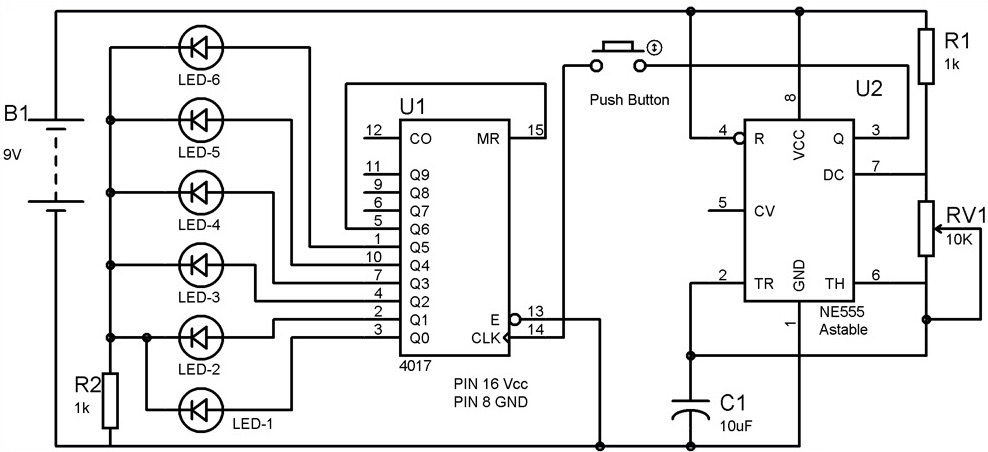
\includegraphics[width=\textwidth]{sch.jpeg}
First, you'll need to know a few keyboard shortcuts. They are listed below. Your mouse must be hovered over the part you want to Rotate, Delete or Move.
\begin{itemize}
	\item A - Add a schematic part
	\item Backspace - Delete a schematic part
	\item R - Rotate a part
	\item M - Move a part
	\item W - Start a wire
	\item K - End a wire
\end{itemize}
\newpage
Now that you know that, we will add the CMOS Chip and 555 Timer. To do this press \textbf{A} on the keyboard. You can type in \textbf{4017} to get the CMOS chip to show up as a Johnson Counter as shown below.
\begin{center}
	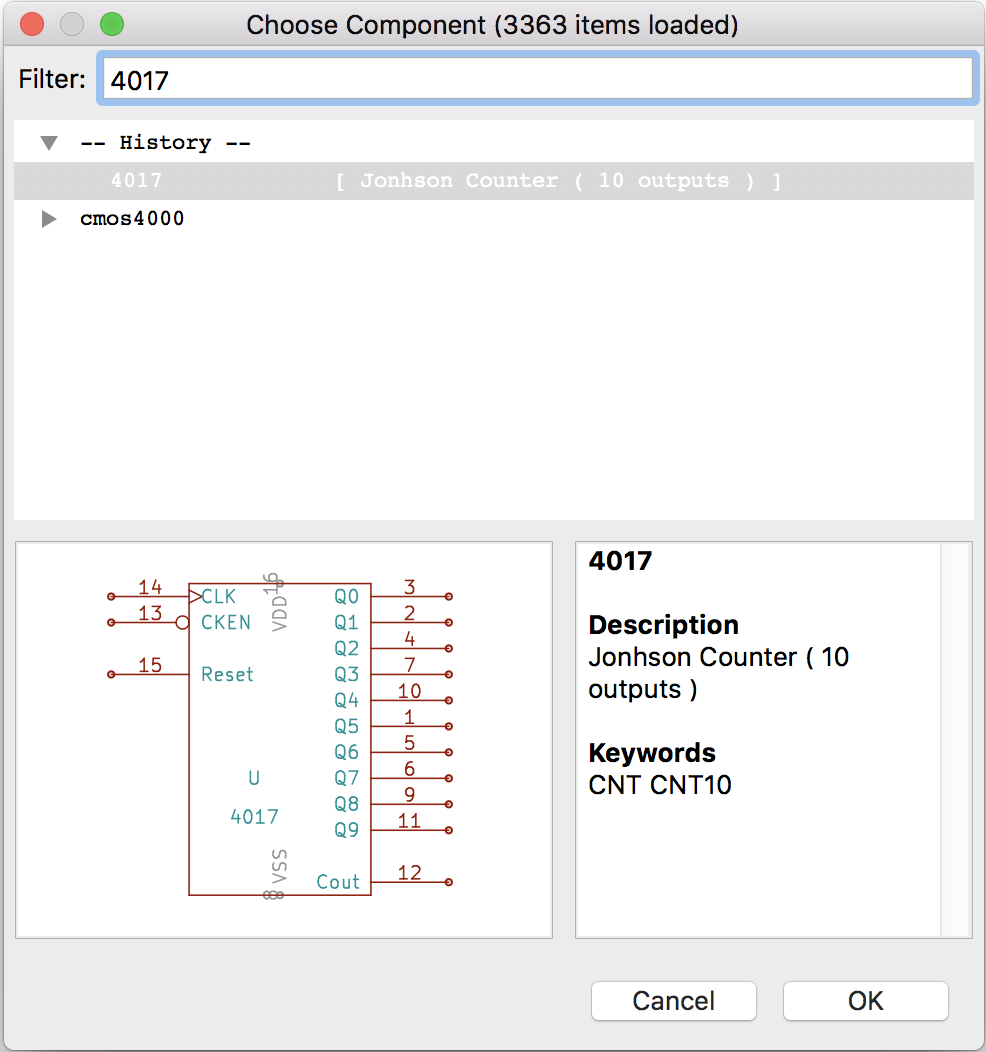
\includegraphics[width=200px]{4017}
\end{center}
Then, click ok and add the part to the schematic by clicking anywhere on the sheet, probably somewhere in the centre is good for this part since we will need to connect things to both sides. Remember we can always move it later!
\\*\\*
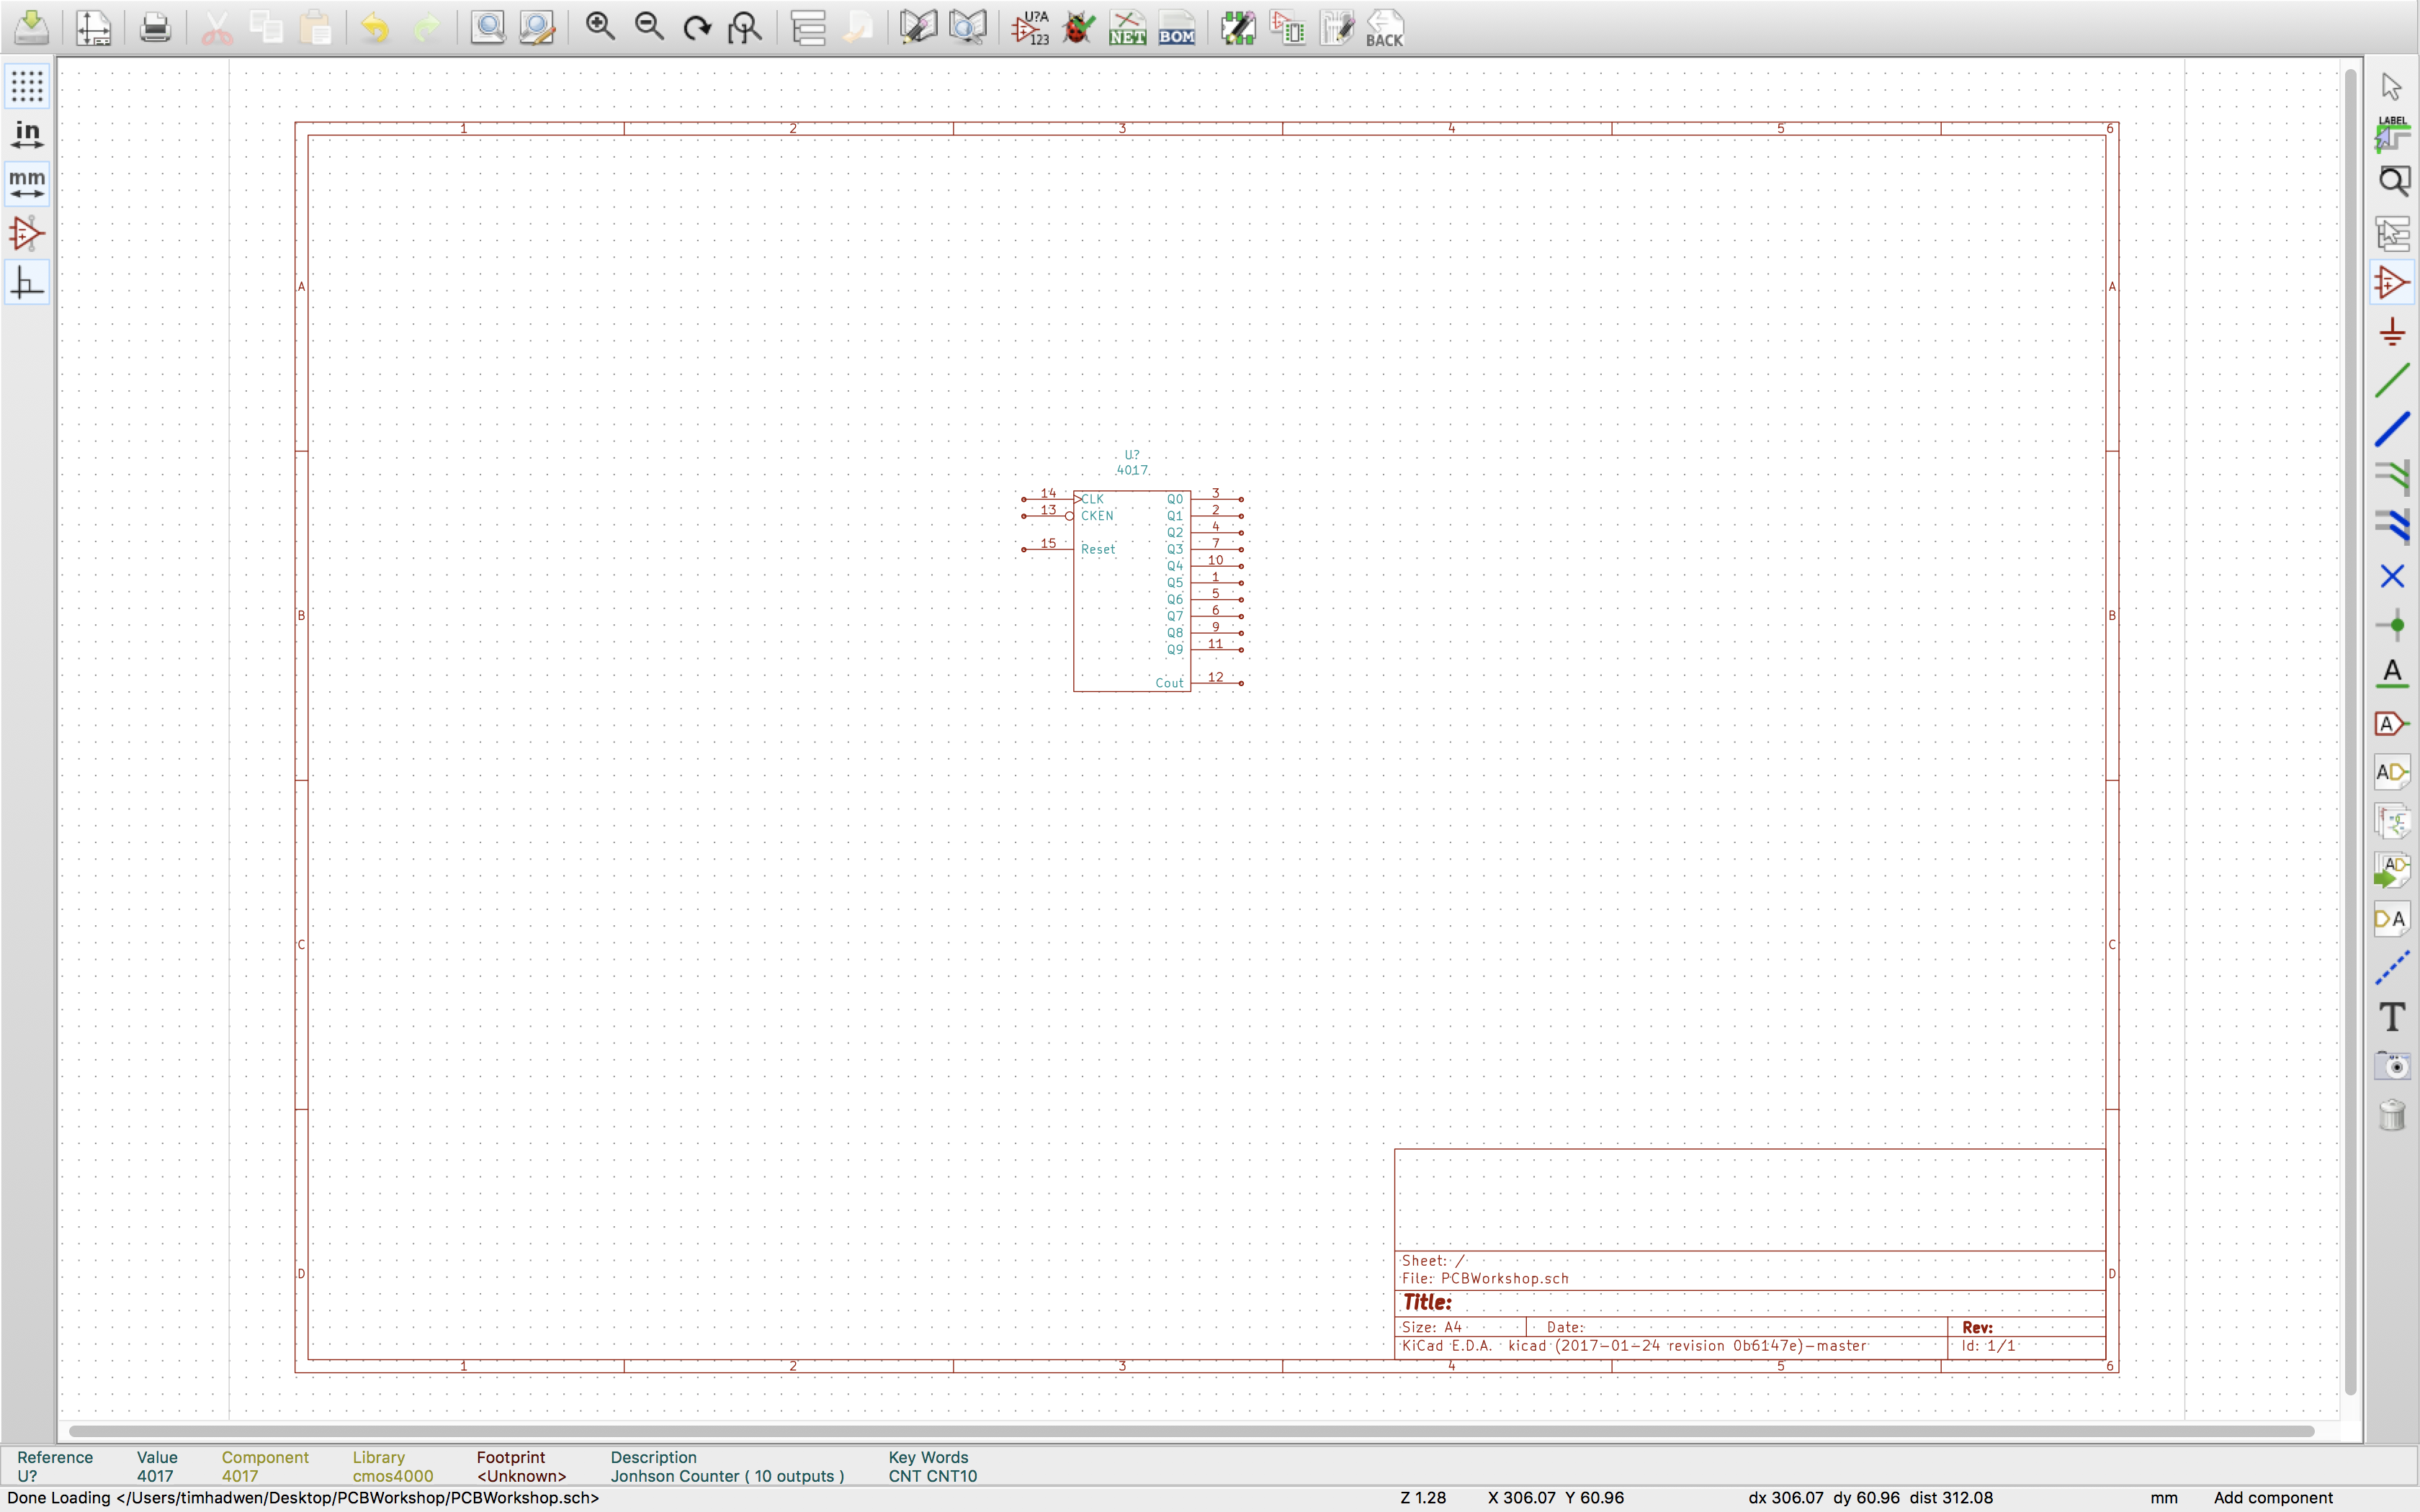
\includegraphics[width=\textwidth]{sch2}
\newpage